
\documentclass[12pt,a4paper]{article}
\usepackage[utf8]{inputenc}
\usepackage[italian]{babel}
\usepackage{geometry}
\usepackage{graphicx}
\usepackage{titlesec}
\usepackage{longtable}
\usepackage{tabularx}
\usepackage{enumitem}
\usepackage{graphicx}
\usepackage{hyperref}
\usepackage{booktabs}
\usepackage{ltablex}
\usepackage[table]{xcolor}
\graphicspath{ {./pictures/} } % definisce la cartella predefinita per le immagini
\usepackage{float}
\geometry{margin=2.5cm}

\begin{document}

% --- PAGINA 1: COPERTINA ---
\begin{titlepage}

    \centering
    \vspace*{2cm}
    {\Huge \textbf{RiciclApp} \par}
    \vspace{1cm}
    {\Large Deliverable D2 \par}
    \vspace{3cm}
    
    {\large \textbf{Gruppo n°:} 20 \par}
    \vspace{1.5cm}
    
    {\large \textbf{Componenti:} \par}
    \vspace{0.5cm}
    \begin{tabular}{rl}
        \textbf{Studente:} & Binco Francesco (Matricola: 243781) \\
        \textbf{Studente:} & Cortese Riccardo (Matricola: 244656) \\
        \textbf{Studente:} & Giovagnetti Lorenzo (Matricola: 247579) \\
    \end{tabular}
    
    \vfill
    {\large Progetto di Ingegneria del Software - Prof. Sandro Luigi Fiore \par}
    \vspace{1.5cm}
    {\large Anno Accademico 2025/2026 \par}
    \vspace{2cm}
\end{titlepage}

% --- PAGINA 2: SOMMARIO ---

\begin{abstract}

Il presente progetto descrive l'ideazione e la progettazione di un sistema per l'ottimizzazione della raccolta differenziata urbana. 

L'obiettivo principale dell'applicazione è duplice: da un lato, semplificare il conferimento dei rifiuti per il cittadino attraverso strumenti di riconoscimento (scansione barcode) e localizzazione dei punti di raccolta con relativo stato di riempimento; dall'altro, fornire agli enti comunali e alle aziende di raccolta una visione d'insieme in tempo reale dello stato del territorio. 

Grazie ai dati trasmessi dai sensori IoT installati nei bidoni, l'amministratore può monitorare i livelli di riempimento, identificare le zone critiche e pianificare interventi di svuotamento mirati. Questo approccio permette di passare da una raccolta a calendario a una gestione dinamica "on-demand", riducendo i costi operativi e l'impatto ambientale dei mezzi di trasporto. 

Il sistema si avvale di una rete di sensori IoT installati nei bidoni stradali per il monitoraggio in tempo reale dei livelli di riempimento, permettendo agli operatori ecologici di usufruire di percorsi di raccolta ottimizzati. 
\end{abstract}


% --- PAGINA 3: INDICE ---
\newpage
\pagenumbering{roman} % Numerazione romana per l'indice
\tableofcontents
\newpage
\pagenumbering{arabic}


\section{Diagramma componenti} 

\subsection{Diagramma dei componenti} 

\begin{figure}[H]
    \centering
    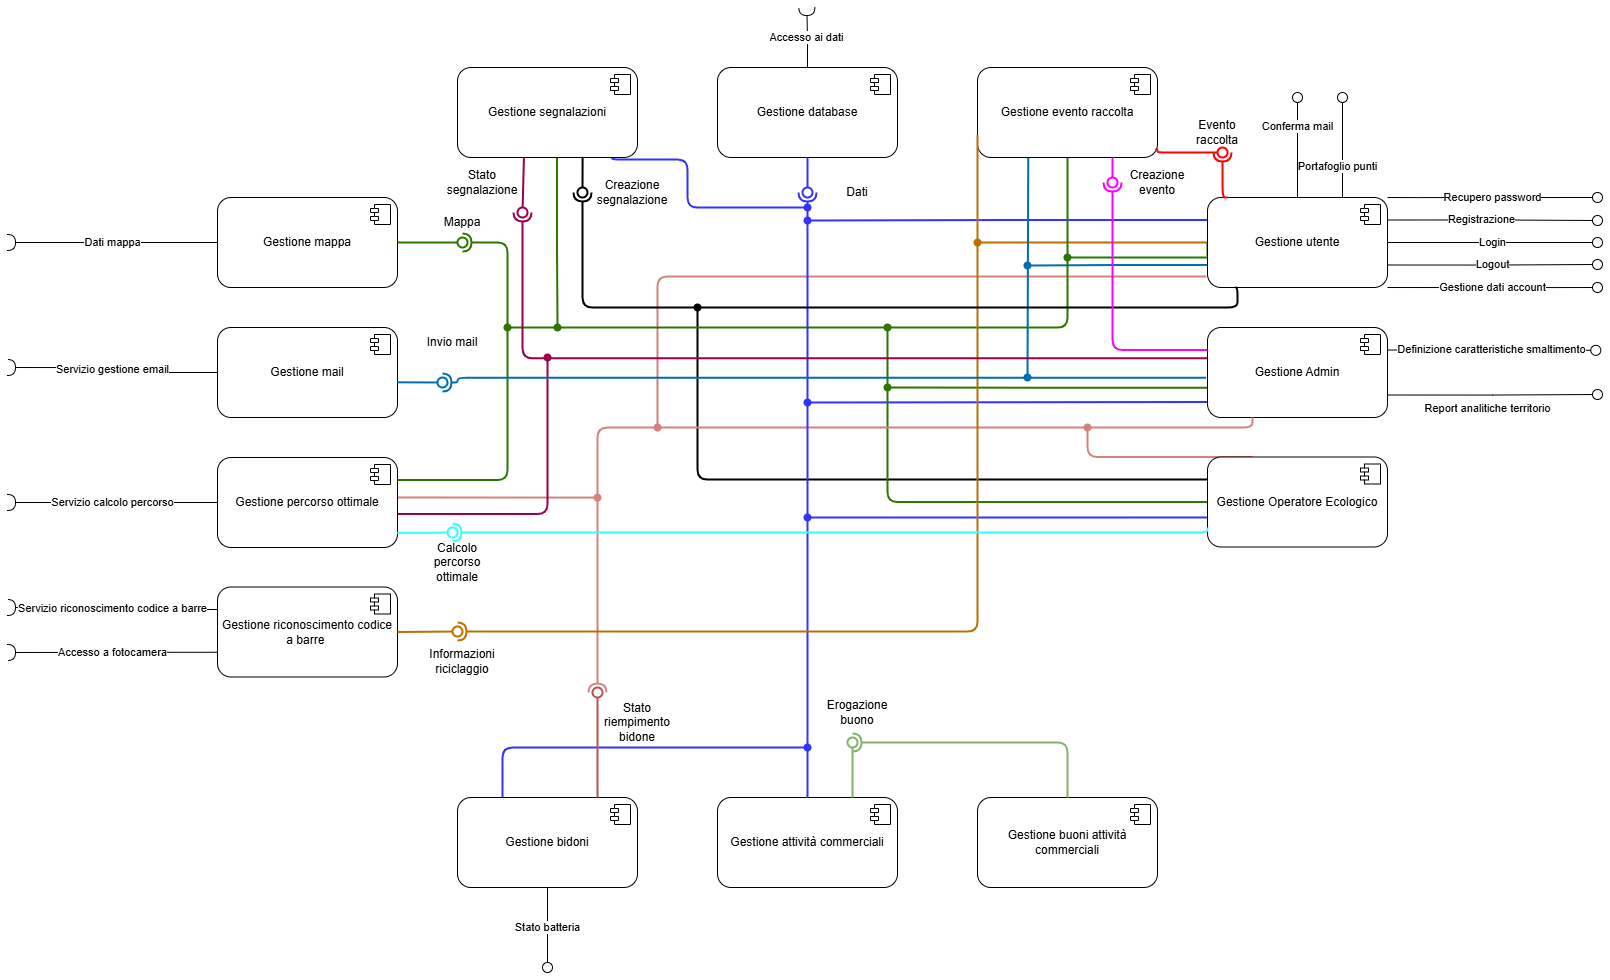
\includegraphics[width=1\linewidth]{diagramma_componenti.png}
    \caption{Diagramma dei componenti}
    \label{fig:placeholder}
\end{figure}

\subsection{Descrizione dei componenti} 
\subsubsection{Gestione utente}
Questo componente permette di gestire tutte le funzionalità richeiste da un utente generico.


\keepXColumns

\begin{tabularx}{\textwidth}{@{}llX@{}}
\caption{Tabelle descrizione componente per gestione utente}
\label{tab:placeholder} \\

\toprule
\textbf{Tipologia} & \textbf{Nome} & \textbf{Descrizione} \\
\midrule
\endfirsthead

\toprule
\textbf{Tipologia} & \textbf{Nome} & \textbf{Descrizione} \\
\midrule
\endhead

\bottomrule
\endfoot

Fornita & Login & Il componente permette ad un utente che in precedenza abbia effettuato una registrazione, quindi in possesso di un account, di effettuare l'accesso tramite username e password \\ \hline

Fornita & Logout & Il componente permette ad un utente che in precedenza abbia effettuato il login, quindi in possesso di un account, di effettuare la disconnessione al proprio account per la sessione in corso \\ \hline

Fornita & Registrazione & Il componente deve permettere ad un utente senza un account associato alla propria mail di creare un account (\textit{RF5}) \\ \hline

Fornita & Recupero password & Il componente deve permettere ad un utente di recuperare la password in caso l'avesse smarrita \\ \hline

Fornita & Conferma mail & Il componente deve permettere ad un utente di confermare la propria mail nel momento in cui esso crea un nuovo account (Registrazione) \\ \hline

Fornita & Portafoglio punti & Il componente tiene traccia di tutti i punti che un utente in possesso di account accumula. Tali punti vengono accreditati in caso di segnalazioni corrette, partecipazioni ad eventi raccolta e per smaltimenti di prodotti (\textit{RF7}). L'utente inoltre può convertire tali punti in buoni sconto offerti dalle attività commerciali (\textit{RF9}) \\ \hline

Fornita & Gestione dati account & Il componente deve permettere all'utente in possesso di account di modificare i dati del proprio account, come ad esempio foto profilo e dati anagrafici (\textit{RF5}) \\ \hline

Richiesta & Dati & Il componente necessita di dati presenti nel database per la gestione dell'utente registrato \\ \hline

Richiesta & Mappa & Il componente necessita di un servizio che permetta di visualizzare la mappa. In questo modo l'utente può visualizzare i centri di raccolta del territorio (\textit{RF1}) \\ \hline

Richiesta & Invio notifica & Il componente necessita di un servizio che permetta di ricevere notifiche nel momento in cui vi siano errori, come ad esempio errori di inserimento di dati \\ \hline

Richiesta & Informazioni riciclaggio & Il componente necessita di un servizio che dia informazioni sul corretto smaltimento di rifiuti tramite il riconoscimento del codice a barre. Il riconoscimento può avvenire tramite scansione dell'immagine oppure tramite inserimento testuale (\textit{RF3, RF4}) \\ \hline

Richiesta & Stato riempimento bidone & Il componente necessita di un servizio che permetta all'utente di viusalizzare lo stato di riempimento dei bidoni nei  vari centri (\textit{RF1, RF2})\\ \hline

Richiesta & Creazione segnalazione & Il componente necessita di un servizio che permetta all'utente di effettuare segnalazioni come ad esempio problemi con bidoni (\textit{RF6}) \\ \hline

Richiesta & Evento raccolta & Il componente necessita di un servizio che permetta all'utente la partecipazione di un evento di raccolta \textit{[nuova aggiunta rispetto a D1}]\\ \hline

Richiesta & Invio mail & Il componente necessita di un servizio che inivii mail in modo che l'utente possa ricevere delle mail come ad esempio per la conferma della mail\\

\end{tabularx}


\subsubsection{Gestione bidoni}
Questo componente permette di gestire le funzionalità per la gestione dei sensori che controllano lo stato di riempimento del bidone.

\keepXColumns

\begin{tabularx}{\textwidth}{@{}llX@{}}
\caption{Tabelle descrizione componente per gestione bidoni}
\label{tab:placeholder} \\

\toprule
\textbf{Tipologia} & \textbf{Nome} & \textbf{Descrizione} \\
\midrule
\endfirsthead

\toprule
\textbf{Tipologia} & \textbf{Nome} & \textbf{Descrizione} \\
\midrule
\endhead

\bottomrule
\endfoot

Fornita & Stato batteria & Il componente permette di visualizzare lo stato della batteria del sistema di controllo del bidone (\textit{RF19}) \\ \hline

Fornita & Stato riempimento bidone & Il componente permette di visualizzare lo stato di riempimento del bidone (\textit{RF19})\\ \hline

Richiesta & Dati & Il componente necessita di dati presenti nel database per la gestione dei vari bidoni disposti nel territorio, come ad esempio posizione o tipologia \\

\end{tabularx}

\subsubsection{Gestione segnalazioni}


\subsubsection{Gestione evento raccolta}

\section{Diagramma delle classi e descrizione delle classi} 
% Documentare almeno 10 classi
In questa sezione viene riportata un'analisi delle classi richieste per implementare il sistema mediante l'utilizzo del diagramma delle classi. Per una maggiore leggibilità viene prima riportato un diagramma complessivo e poi un'analisi su alcuni gruppi di classi. Per ogni classe/le classi principali vengono specificati attributi e operazioni (descrizione, parametri e valori di ritorno).

% Documentare:
%- diagramma delle classi completo o in parti
%- Per ogni classe/gruppo di classi che si decide di analizzare, viene riportata una breve descrizione di ciascuna classe (inclusi i suoi metodi).

\subsection{Diagramma delle classi} 
% Inserire qui il diagramma completo o in parti
La Figura~\ref{fig:diagramma-classi} mostra il diagramma delle classi del sistema RiciclApp.

\begin{figure}[H]
    \centering
    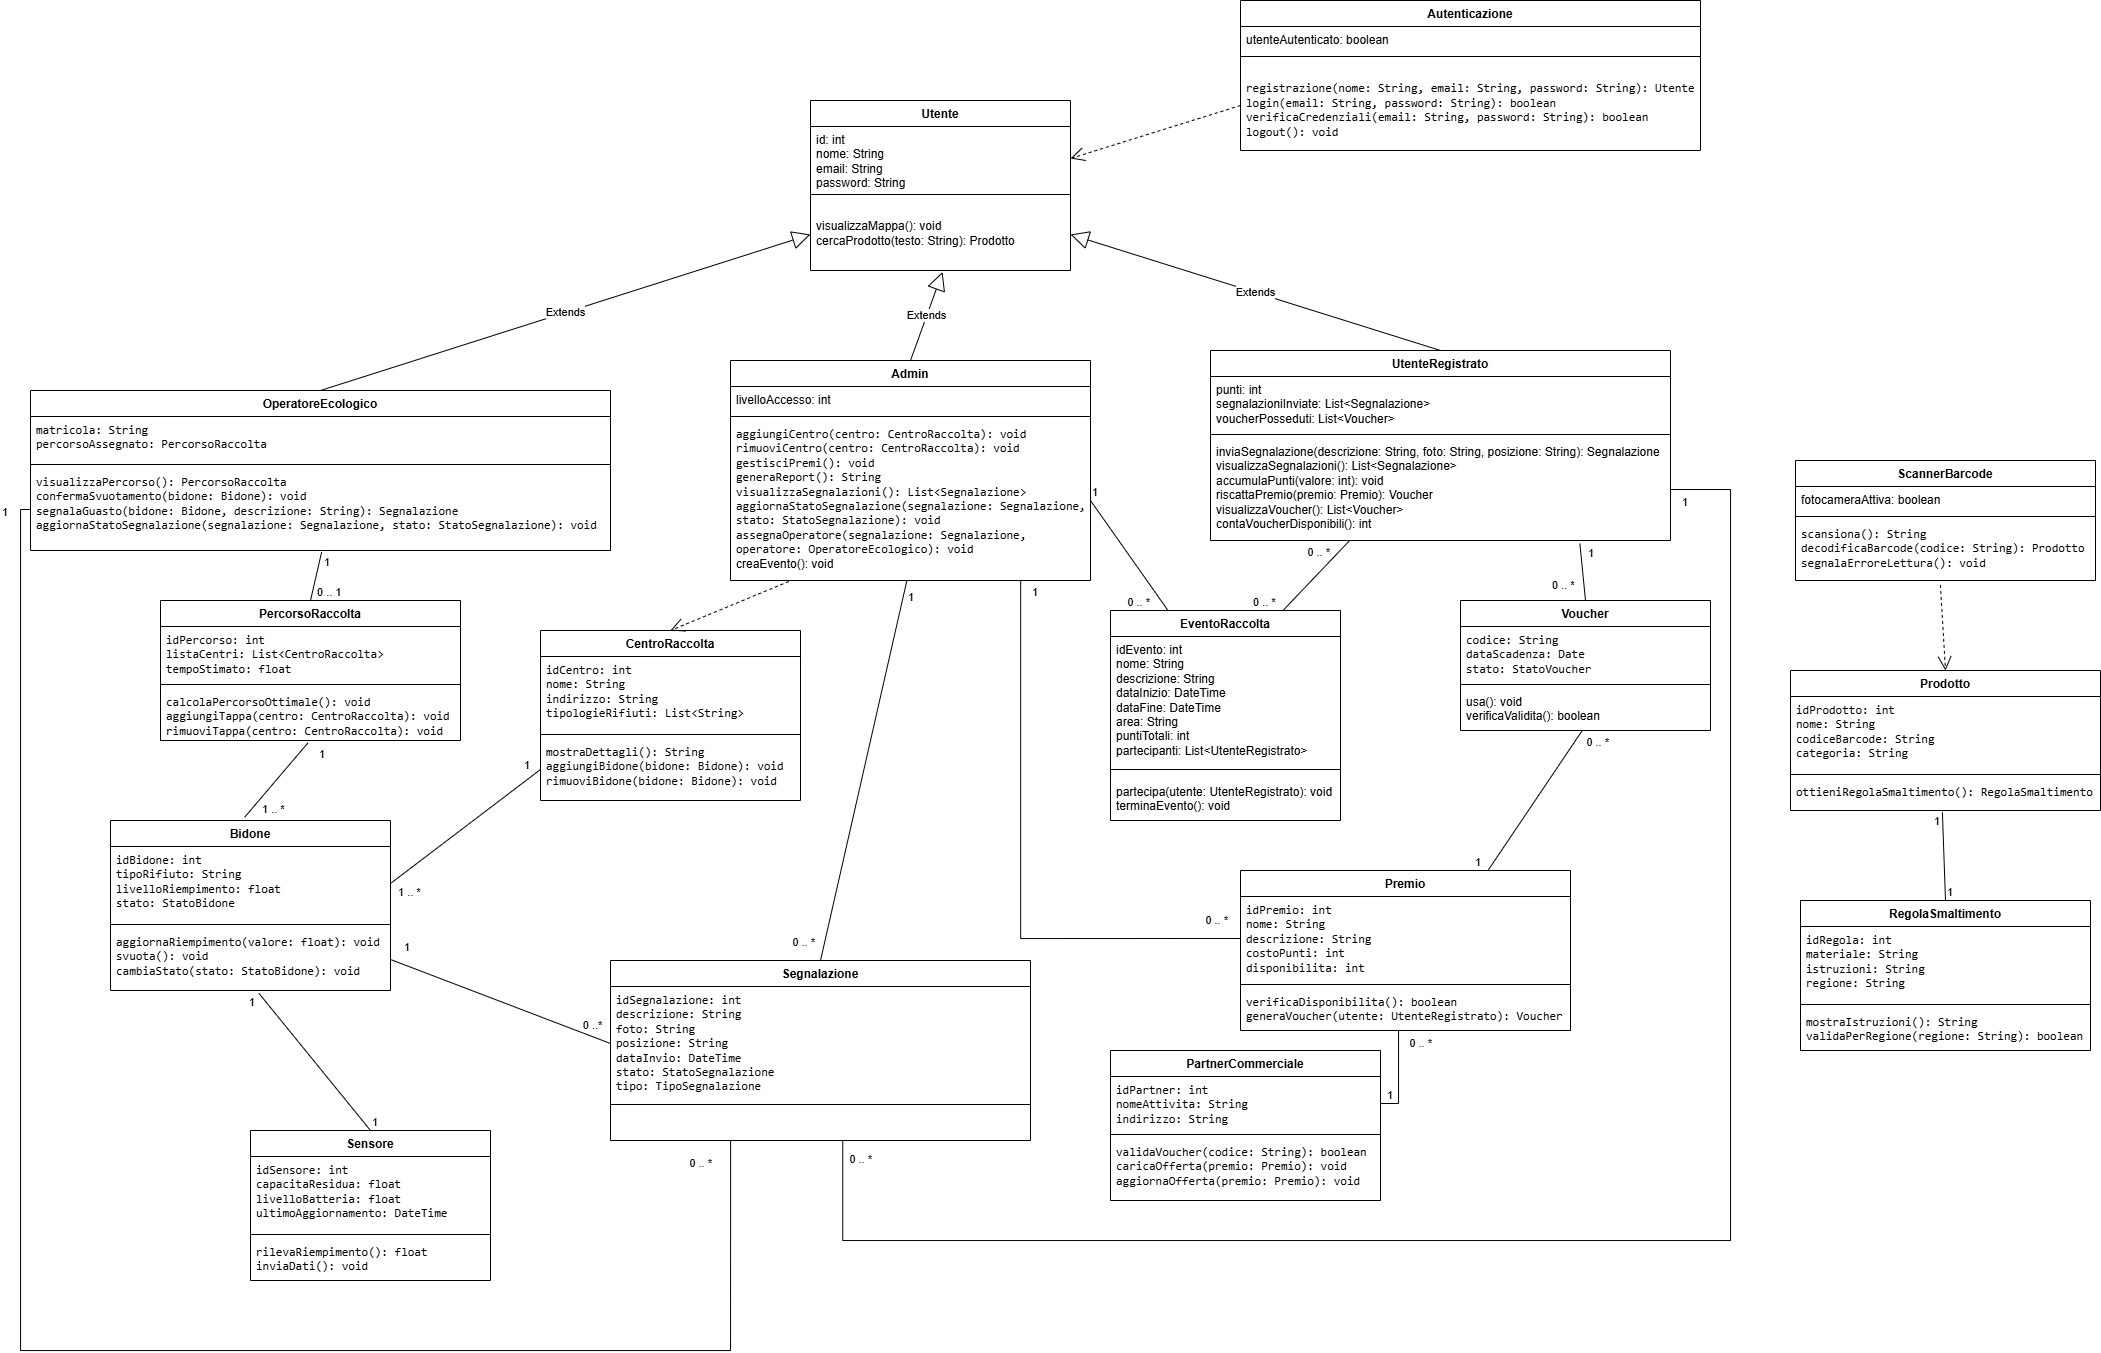
\includegraphics[width=\textwidth]{diagramma_uml_classi.png}
    \caption{Diagramma delle classi di RiciclApp}
    \label{fig:diagramma-classi}
\end{figure}

\subsection{Gruppo classi autenticazione e profilo} 
Vengono analizzate qui le classi che si occupano della gestione dell'autenticazione e del profilo utente.

\subsubsection{Gestione Autenticazione} 
Questa classe si occupa principalmente della gestione del login e della registrazione dell'utente. I suoi attributi sono quindi i dati relativi all'utente che vengono utilizzati per verificare la corrispondenza con i dati nel database.

\begin{table}[h]
\begin{tabular}{@{}ll@{}}
\toprule
\textbf{Operazione}  & \textbf{Descrizione}  \\ \midrule
impostaValori()  & legge i valori immessi in input dall'utente e li salva nei  \\
 & corrispettivi attributi. \\ \bottomrule
\end{tabular}
\end{table}

\section{Constraint OCL} 
% Riportare almeno 10 - 12 constraint OCL (incluse invarianti, precondizioni, postcondizioni): una breve descrizione e il constraint
In questa sezione vengono analizzati in linguaggio OCL i vincoli legati al diagramma delle classi. Questi vincoli rappresentano invarianti, precondizioni e postcondizioni sulle operazioni delle classi.

\subsection{Classe Gestione Autenticazione} 
\textbf{Descrizione:} l'operazione login (String username, String password) setta l'attributo autenticato a true.

\begin{quote}
\texttt{context GestionAutenticazione::login (username, password): boolean}  \\
\texttt{post: autenticato = true} 
\end{quote}

\end{document}
